
\section{Resoconto attività di verifica}

\subsection{Verifica documentazione}
 Come descritto nelle \dext{norme di progetto}, vengono usate la tecnica del  \glock{walkthrough} per la validazione dei vari documenti con cadenza periodica, per una verifica generale dell'adempimento a tutte le regole, e della tecnica dell' \glock{inspection} per la verifica delle varie modifiche/aggiunte ai documenti

\subsubsection{Calcolo leggibilità documenti}
Come descritto nelle \dext{norme di progetto}, si utilizza \glock{l'indice di Gulpease} per la verifica che i documenti siano leggibili e comprensibili da tutti. 
Di seguito viene riportato il grafico contenente i risultati ottenuti durante il periodo di analisi dei requisiti nei 6 periodi definiti:

\begin{figure}[H]
	\centering
	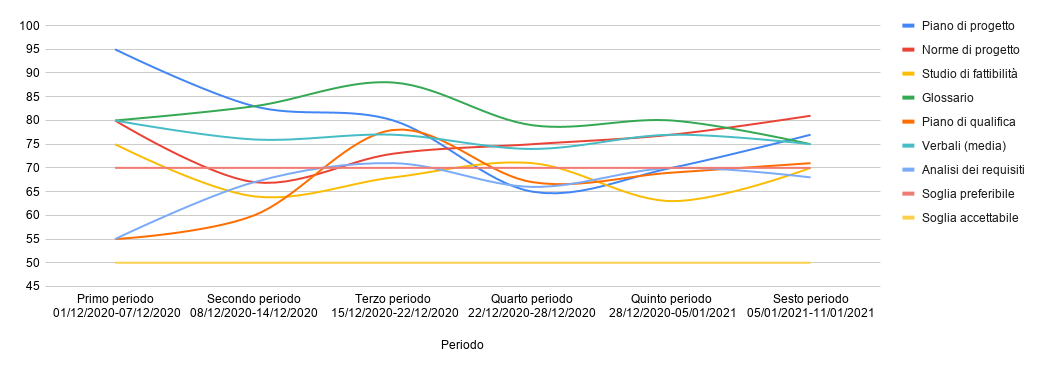
\includegraphics[width=0.8\linewidth]{./res/images/gulpease.png}
	\caption{Grafico periodo/indice di Gulpease nel periodo di analisi dei requisiti}
	\label{fig:Grafico indice di Gulpease periodo di analisi dei requisiti}
\end{figure}

\subsubsection{Calcolo ortografia documenti}
Di seguito riportati risultati dei controlli periodici dei vari documenti riguardo a errori ortografici nel periodo di analisi dei requisiti:
\begin{figure}[H]
	\centering
	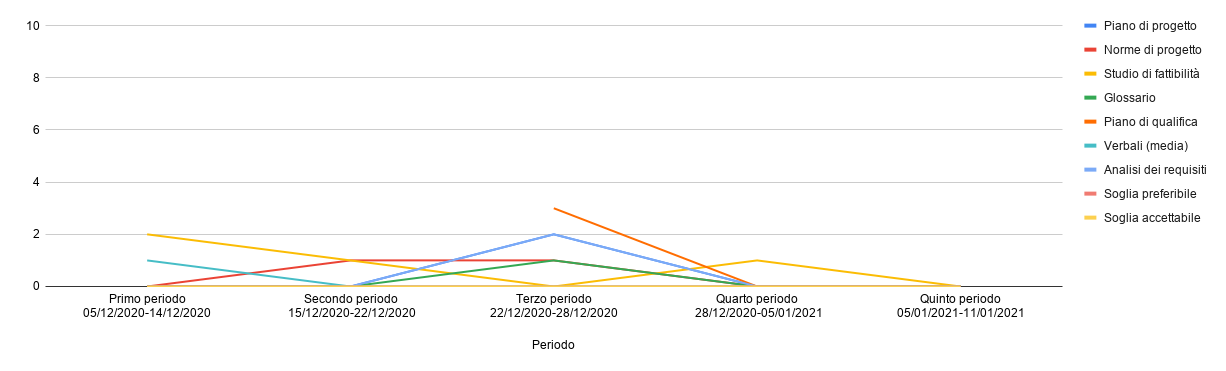
\includegraphics[width=0.8\linewidth]{./res/images/ortografia.png}
	\caption{Grafico periodo/errori ortografici nel periodo di analisi dei requisiti}
	\label{fig:Grafico errori ortografici periodo di analisi dei requisiti}
\end{figure}

Condizione documenti finali:
\begin{center}
	\rowcolors{2}{lightest-grayest}{white}
	\begin{longtable}{|c|c|c|}
	\hline
	\rowcolor{lighter-grayer}
	\textbf{Documento} & \textbf{Errori ortografici} & \textbf{Accettabile} \\
	\hline
	\endfirsthead

	\hline
	Piano di Progetto & 0 & Sì \\
	\hline
	\hline
	Norme di Progetto &  0 & Sì \\
	\hline
	\hline
	Studio di fattibilità & 0 & Sì \\
	\hline
	\hline
	Glossario & 0 & Sì \\
	\hline
	\hline
	Piano di qualifica & 0 & Sì \\
	\hline
	\hline
	Media verbali & 0 & Sì \\
	\hline
	\hline
	Analisi dei requisiti & 0 & Sì \\
	\hline
	\rowcolor{white}
	\caption{Tabella delle medie degli errori di ortografia durante il periodo di analisi dei requisiti}
	\end{longtable}
\end{center}
